%%% LaTeX Template: Article/Thesis/etc. with colored headings and special fonts
%%%
%%% Source: http://www.howtotex.com/
% vim: set spell spelllang=es syntax=tex :

\documentclass[12pt]{article}
\usepackage{styles/apuntes-estilo}
\usepackage{fancyhdr,lastpage}
\usepackage{hyperref}
\usepackage[inline]{enumitem}
\usepackage{xurl}
\usepackage{nameref}
\usepackage{tabularx}

\usepackage{appendix}
\renewcommand{\appendixname}{Anexo}
\renewcommand{\appendixtocname}{Anexo}
\renewcommand{\appendixpagename}{Anexo}

\newcommand{\multiline}[2][c]{
      \begin{tabular}[#1]{@{}c@{}}#2\end{tabular}
      }

\def\maketitle{

\makeatletter{
    \color{blue} \centering \huge \sc
    \textbf{
        Trabajo práctico N° 7\\
        \large \vspace*{-8pt} \color{black}
        El software
        \vspace*{8pt}
    }\\
    \small Fecha de finalización: 24 de Mayo
    \par
}

\makeatother

\makeatletter
% vim: set spell spelllang=es syntax=tex :
 {\centering \small 
    Introducción a la computación\\
    Departamento de Ingeniería de Computadoras \\
    Facultad de Informática - Universidad Nacional del Comahue \\
    \vspace{20pt} }
\makeatother

\vspace{-2.5cm}
\mbox{\hspace{-1cm}\includegraphics[width=3cm,height=3cm]{logos/uncoma.pdf}\hspace{12cm}
    
\includegraphics[width=3cm,height=3cm]{logos/fai.pdf}}



}

% Custom headers and footers
\fancyhf{} % clear all header and footer fields
\fancypagestyle{plain}{\fancyhf{}}
\pagestyle{fancy}
\lhead{\footnotesize TP N° 7 - El Software}
\rhead{\footnotesize \thepage\ }

\def\ti#1#2{\texttt{#1} & #2 \\ }

\begin{document}

\thispagestyle{empty}
\maketitle
\setlength{\parindent}{1pt}

\textbf{Objetivo:} Comprender la organización y el funcionamiento básico de
una computadora simple. Se involucran conocimientos de los componentes
hardware y sus interacciones para ejecutar instrucciones.

\textbf{Recursos bibliográfico:}

\vspace{-2\topsep}
\begin{itemize}

    \itemsep2pt \parskip0pt \parsep0pt

    \item \emph{Andrew S. Tanenbaum}. Organización de computadoras: un enfoque
        estructurado. Cuarta edición, editorial Pearson Educación, 2000. ISBN
        970-170-399-5.

\end{itemize}

\textbf{Lectura obligatoria:}

\vspace{-2\topsep}
\begin{itemize}

    \itemsep2pt \parskip0pt \parsep0pt

    \item Apuntes de cátedra. \emph{Capitulo 5: Arquitectura y Organización de
        Computadoras}, y \emph{Capitulo 7: El Software}. Disponible en:
        \url{https://egrosclaude.github.io/IC/IC-notes.pdf}

\end{itemize}

\section*{Modelo Computacional Binario Elemental (MCBE)}

\begin{enumerate}
    \itemsep2pt \parskip0pt \parsep0pt

    \item ¿Qué es organización de una computadora y que es su arquitectura?

    \item ¿Cuáles son las componentes de una CPU? ¿Cuáles son las componentes
        de una computadora?

    \item ¿Qué diferencias entre los registros y la memoria principal?

    \item Si una nueva arquitectura tiene instrucciones con 5 bits para el
        código de operación y 10 para operando (donde en el caso de las
        instrucciones de carga y almacenamiento indican la dirección de la
        celda origen o destino) ¿Cuantas operaciones distintas puede tener
        como máximo esta arquitectura? ¿Cuantas celdas de memoria puede tener?

    \item Se desea establecer el tamaño mínimo para una arquitectura que tiene
        14 instrucciones distintas. Cada instrucción tiene tres operandos, y
        cada operando referencia una de las 512 celdas de memoria ¿Cuál es la
        cantidad mínima de bits que puede tener una instrucción?

    \item Con respecto a la memoria de la \emph{MCBE}, indique:

        \begin{enumerate}

            \item Cantidad de celdas de memoria.

            \item Tamaño de una celda de memoria en \emph{bits}
                y \emph{bytes}.

            \item Tamaño total en \emph{bytes}.

            \item Dirección de la primera y de última celda de memoria.

            \item ¿Para qué se utilizan las direcciones \textbf{30} y
                \textbf{31}? ¿Qué dispositivos podrían conectarse en esas
                direcciones?

        \end{enumerate}

    \item Con respecto a la \emph{CPU} de la \emph{MCBE}, indique:

        \begin{enumerate}

            \item Registros y sus propósitos.

            \item ¿Qué representación y tamaño (en \emph{bits}) de números
                utilizan las instrucciones aritméticas? ¿Cuál es el rango de
                valores del acumulador?

        \end{enumerate}

    \item Con respecto a las instrucciones ejecutadas por la \emph{CPU} de la
        \emph{MCBE}, indique:

        \begin{enumerate}

            \item ¿A qué distancia máxima puede ``saltar'' el control del
                programa?

            \item ¿Puede el \emph{MCBE} encontrar una instrucción que no sea
                capaz de decodificar?

            \item ¿Qué pasa si el programa no contiene una instrucción
                \emph{HLT}?

        \end{enumerate}

\end{enumerate}

\appendix
\clearpage
\addappheadtotoc
\appendixpage

\section*{Descripción del Modelo Computacional Binario Elemental (MCBE)}

\begin{description}
    \itemsep2pt \parskip0pt \parsep0pt

    \item[Memoria:] consta de 32 posiciones de 8 bits. Las direcciones 0 a 29
        corresponden a direcciones que pueden ser escritas y leídas. La
        dirección 30 es de \textbf{sólo lectura}, permite leer datos del
        dispositivo de entrada, por ejemplo un teclado. La dirección 31 es de
        \textbf{sólo escritura}, permite escribir datos en el dispositivo de
        salida, por ejemplo en una pantalla o una impresora.

    \item[Registro PC:] registro de 8 bits, contiene la dirección de la
        próxima instrucción a ejecutar. Se inicializa en cero.

    \item[Registro IR:] registro 8 bits donde se guarda la instrucción que se
        esta decodificando o ejecutando.

    \item[Registro acumulador:] registro de 8 bits donde se almacena un
        número entero representado en \emph{complemento a 2}.

    \item[Etiquetas predefinidas:]~

        \begin{description}
            \itemsep2pt \parskip0pt \parsep0pt

            \item[IN:] dirección 30, entrada, dirección de solo lectura.

            \item[OUT:] dirección 31, salida, dirección de solo escritura.

        \end{description}

    \item[Instrucciones:] de 8 bits, los 3 bits más significativos almacenan
        el código de operación, y los 5 menos significativos almacenan el
        operando.

        \begin{figure}[h]
            \centering
            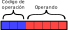
\includegraphics[height=4em]{img/instruccion.pdf}
        \end{figure}

\end{description}

\begin{tabularx}{\textwidth}{c|c|c|X}

    \textbf{Mnemónico/Dato} & \textbf{Código de} & \textbf{Operando} &
    \multicolumn{1}{c}{\textbf{Descripción}} \\

    & \textbf{operación} & & \\

    & \emph{3 bits} & \emph{5 bits} & \\
    \hline
    \hline

    \texttt{LD} & 010 & \emph{dirección} & \textbf{Memoria → Acumulador}. Copia
    un byte desde la dirección de memoria al acumulador. \\ \hline

    \texttt{ST} & 011 & \emph{dirección} & \textbf{Acumulador → Memoria}. Copia
    el contenido del acumulador en esa dirección de memoria. \\ \hline

    \texttt{ADD} & 100 & \emph{dirección} & \textbf{Suma}. El contenido de la
    dirección se suma al acumulador, y el resultado se almacena en el
    acumulador. \\ \hline

    \texttt{SUB} & 101 & \emph{dirección} & \textbf{Resta}. El contenido de la
    dirección se resta al acumulador, y el resultado se almacena en el
    acumulador. \\ \hline

    \texttt{JMP} & 110 & \emph{desplazamiento} & \textbf{Salto incondicional}. Se
    suma (en complemento a 2) el desplazamiento al \textbf{PC}. \\ \hline

    \texttt{JZ} & 111 & \emph{desplazamiento} & \textbf{Salto condicional}. Si
    el acumulador es cero, se suma (en complemento a 2) el desplazamiento al
    \textbf{PC}, en caso contrario el \textbf{PC} se incrementa en uno. \\
    \hline

    \texttt{HLT} & 001 & \emph{(sin uso)} & \textbf{Detiene la maquina}. No se
    ejecutan nuevas instrucciones. Los registros y la memoria quedan con el
    último valor que tenían. \\ \hline

    \texttt{NOP} & 000 & \emph{(sin uso)} & \textbf{No operación}. No tiene
    ningún efecto sobre el acumulador ni memoria. El \textbf{PC} se incremente
    en uno. \\

\end{tabularx}

\end{document}
